\documentclass[10pt]{article}

% AAAI-27 note:
% Replace this lightweight article preamble with the official AAAI-27 author kit
% as soon as it is released. The content below is intentionally style-agnostic.
\usepackage[margin=0.9in]{geometry}
\usepackage{times}
\usepackage{microtype}
\usepackage{amsmath,amssymb,amsfonts}
\usepackage{booktabs}
\usepackage{graphicx}
\usepackage{subcaption}
\usepackage{multirow}
\usepackage{xcolor}
\usepackage{enumitem}
\usepackage{algorithm}
\usepackage{algpseudocode}
\usepackage[numbers,sort&compress]{natbib}
\usepackage[colorlinks=true,linkcolor=blue,citecolor=blue,urlcolor=blue]{hyperref}

\graphicspath{{figures/}}
\setlength{\textfloatsep}{8pt plus 2pt minus 2pt}
\setlength{\floatsep}{8pt plus 2pt minus 2pt}
\setlength{\intextsep}{8pt plus 2pt minus 2pt}
\setlist[itemize]{leftmargin=*,topsep=2pt,itemsep=1pt}

\newcommand{\ours}{F-CS-WAE}
\newcommand{\simple}{CS-WAE}
\newcommand{\zc}{z_{\mathrm{c}}}
\newcommand{\zs}{z_{\mathrm{s}}}
\newcommand{\Sph}{\mathbb{S}}
\newcommand{\R}{\mathbb{R}}

\title{\vspace{-1.0em}
F-CS-WAE: Factorized Class-Structured Spherical Cauchy Wasserstein Auto-Encoders
for Label-Guided Generative Clustering
\vspace{-0.3em}}

\author{
Anonymous Authors\\
\small Anonymous Institution\\
\small \texttt{anonymous@example.com}
}

\date{}

\begin{document}
\maketitle

\begin{abstract}
Generative clustering requires a latent space that is simultaneously discriminative, reconstructive, and samplable. These requirements often conflict: a representation can form clean clusters while decoding poor prior samples, or reconstruct images accurately while providing little class structure. We study this tension through \ours, a factorized class-structured Wasserstein auto-encoder that separates a hyperspherical semantic latent $\zc\in\Sph^{d_{\mathrm{c}}-1}$ from a Euclidean style latent $\zs\in\R^{d_{\mathrm{s}}}$. The semantic component is regularized by class-conditional Spherical Cauchy priors on the hypersphere, while the style component is matched to a Gaussian prior using MMD. A four-phase schedule first learns reconstruction, then gradually introduces style matching, auxiliary semantic classification, and semantic prior alignment. On CIFAR-10, \ours achieves $80.87\pm0.52\%$ clustering accuracy over three seeds with FID $83.04\pm0.86$, substantially improving over available VAE, WAE-MMD, VaDE, and single-latent baselines under the repository protocol. On MNIST, \ours reaches $99.15\%$ clustering accuracy and strong reconstruction quality, but a diagnostic analysis reveals a conditional prior mismatch: the global style aggregate resembles $N(0,I)$, yet style codes remain class-dependent, causing naive independent prior samples to decode poorly. This failure mode is not incidental; it exposes a central design issue in factorized generative clustering. We therefore present \ours as both a strong empirical model and a diagnostic framework for studying when semantic/style factorization improves or harms sampling. The current evidence suggests that AAAI-level claims should combine clustering gains with conditional style alignment, rather than relying on clustering metrics alone.
\end{abstract}

\section{Introduction}

Auto-encoding generative models promise a compact latent representation from which one can reconstruct inputs, sample new data, and analyze structure. In clustering-oriented settings, however, these goals pull the model in different directions. Reconstruction rewards retaining all information needed to reproduce an image. Clustering rewards removing nuisance variation and preserving class-relevant structure. Prior sampling rewards matching the encoded distribution to a simple distribution from which new latent codes can be drawn. A model that optimizes one of these objectives can easily fail another.

This tension is visible in variational auto-encoders (VAEs) \citep{kingma2013autoencoding}, Wasserstein auto-encoders (WAEs) \citep{tolstikhin2017wasserstein}, and deep generative clustering methods such as VaDE \citep{jiang2016variational}. VAEs provide a probabilistic latent-variable model, but their Euclidean Gaussian priors do not automatically form class-separated representations. WAEs match the aggregated posterior to a prior, often using MMD, but global matching alone does not impose semantic organization. VaDE introduces a Gaussian mixture prior for clustering, yet it remains Euclidean and does not explicitly separate class semantics from within-class style.

Hyperspherical latent variables offer a natural alternative for semantic organization. If class identity is encoded primarily by direction, then points on a unit sphere can be compared angularly and organized around class centers. Hyperspherical VAEs \citep{davidson2018hyperspherical} and Spherical Cauchy VAEs \citep{sablica2025hyperspherical} show that distributions on the sphere can be used in deep generative models. The single-latent \simple{} model in this repository uses this idea: one spherical latent variable is matched to class-conditional Spherical Cauchy priors. It generates relatively clean MNIST samples, but its clustering performance is limited compared with the factorized model studied here.

We introduce \ours, a factorized class-structured Spherical Cauchy WAE. The model decomposes the latent representation into two parts. The semantic latent $\zc$ lives on a hypersphere and is aligned with class-conditional Spherical Cauchy priors. The style latent $\zs$ lives in Euclidean space and is regularized toward a Gaussian prior. The architecture is motivated by a simple hypothesis: class identity should be represented by hyperspherical directions, while residual appearance variation should be carried by a separate style code.

The empirical picture is nuanced. On CIFAR-10, the factorized model dramatically improves clustering over available baselines and maintains substantially better sample quality than the older single-latent ResNet variant. On MNIST, it obtains almost perfect clustering and excellent reconstructions, but naive prior samples are worse than those of \simple{}. A targeted diagnostic shows why: $\zs$ is globally matched to a Gaussian, but remains conditionally dependent on class. Thus, sampling $\zc$ from a class prior and $\zs$ independently from $N(0,I)$ creates latent pairs that the decoder did not learn to map to realistic images.

This paper is therefore written with a conservative claim. \ours{} is a strong factorized model for label-guided clustering, and its failure mode is scientifically useful: it identifies conditional style mismatch as a central obstacle for making factorized WAE models simultaneously cluster-friendly and sample-friendly. For a final AAAI-27 submission, we argue that the correct target is not merely higher ACC/NMI/ARI, but a factorized objective that preserves clustering gains while repairing conditional decoding.

\paragraph{Contributions.}
\begin{itemize}
    \item We formulate \ours, a factorized class-structured WAE with a Spherical Cauchy semantic latent and a Gaussian style latent.
    \item We introduce a four-phase training schedule that separates reconstruction learning, style regularization, semantic supervision, and class-prior alignment.
    \item We provide repository-local empirical evidence on CIFAR-10 and MNIST, including multi-seed CIFAR-10 results and a direct comparison against a single-latent \simple{} variant.
    \item We diagnose a conditional prior mismatch in the MNIST model, showing that global style MMD is insufficient for reliable class-conditional generation.
    \item We outline the method extension required for an AAAI-27-strength paper: conditional style priors and per-class style matching.
\end{itemize}

\section{Position in the Field}

\paragraph{Auto-encoding generative models.}
VAEs \citep{kingma2013autoencoding} optimize an evidence lower bound with a KL penalty between approximate posteriors and a latent prior. WAEs \citep{tolstikhin2017wasserstein} instead minimize reconstruction loss plus a discrepancy between the aggregated posterior and a target prior. This makes WAEs attractive for generative representation learning: the regularizer explicitly encourages encoded samples to be drawn from a distribution that is easy to sample. MMD-based WAEs use kernel two-sample distances \citep{gretton2012kernel} as the discrepancy.

\paragraph{Generative clustering.}
Deep Embedded Clustering \citep{xie2015unsupervised} and VaDE \citep{jiang2016variational} connect latent-variable modeling with clustering. VaDE in particular uses a Gaussian mixture prior, making cluster assignment part of the generative model. \ours{} differs in two respects. First, it is label-guided rather than fully unsupervised: class labels are used during training to structure the semantic prior. Second, it uses hyperspherical semantic geometry rather than a Euclidean mixture.

\paragraph{Hyperspherical and heavy-tailed latent variables.}
Hyperspherical VAEs \citep{davidson2018hyperspherical} motivate distributions on $\Sph^{d-1}$ when directional geometry is important. Spherical sliced-Wasserstein distances \citep{bonet2022spherical} adapt distribution matching ideas to spheres. Spherical Cauchy VAEs \citep{sablica2025hyperspherical} further provide an efficient Mobius-transform reparameterization. \ours{} uses this family for the semantic latent, but combines it with WAE-style MMD and label-guided class priors.

\paragraph{Factorization and disentanglement.}
Factorized latent spaces have a long history in disentanglement. InfoGAN \citep{chen2016infogan} uses mutual information to make selected latent codes interpretable. FactorVAE \citep{kim2018disentangling} and $\beta$-TCVAE \citep{chen2018isolating} penalize total correlation to encourage independent factors. These works motivate our central diagnostic: if semantic and style variables are intended to factorize, then matching only the marginal style distribution is insufficient. One must also control dependence between style and class or between style and semantic latents.

\paragraph{Where \ours{} fits.}
\ours{} sits between generative clustering and disentangled representation learning. Its semantic latent is explicitly class-structured, like a supervised version of mixture-prior clustering. Its style latent is intended to capture residual variation. Unlike purely disentangled VAEs, however, \ours{} is evaluated not by interpretability alone but by clustering, reconstruction, and prior sampling. This combined evaluation is important because it exposes a failure mode that a clustering-only table would hide.

\section{Method}

\subsection{Problem Setting}

Let $\mathcal{D}=\{(x_i,y_i)\}_{i=1}^{n}$ be a labeled image dataset with $K$ classes. The goal is to learn a generative representation that supports:
\begin{enumerate}
    \item reconstruction: $x\mapsto \hat{x}$ should preserve visual content;
    \item clustering: a simple clustering method on semantic codes should recover class structure;
    \item sampling: latent samples from the prior should decode into realistic class-conditional images.
\end{enumerate}
We call the setting \emph{label-guided generative clustering}. Labels are used during training to organize the prior, but evaluation of clustering uses K-means and Hungarian matching on latent codes.

\subsection{Architecture}

\ours{} uses a shared convolutional encoder with two heads:
\begin{equation}
    E_\phi(x) = (\tilde{\mu}_{\mathrm{c}}, r_{\mathrm{c}},
    \mu_{\mathrm{s}}, \log\sigma_{\mathrm{s}}^2).
\end{equation}
The semantic direction is normalized,
\begin{equation}
    \mu_{\mathrm{c}} =
    \frac{\tilde{\mu}_{\mathrm{c}}}{\|\tilde{\mu}_{\mathrm{c}}\|_2},
    \qquad
    \rho_{\mathrm{c}} = \sigma(r_{\mathrm{c}})(1-\epsilon),
\end{equation}
where $\mu_{\mathrm{c}}\in\Sph^{d_{\mathrm{c}}-1}$ and $\rho_{\mathrm{c}}\in(0,1)$. A semantic latent is sampled by a Spherical Cauchy Mobius reparameterization,
\begin{equation}
    \eta_{\mathrm{c}}\sim \mathrm{Unif}(\Sph^{d_{\mathrm{c}}-1}),
    \qquad
    \zc = T_{\mu_{\mathrm{c}},\rho_{\mathrm{c}}}(\eta_{\mathrm{c}}).
\end{equation}
The style latent uses a Gaussian reparameterization,
\begin{equation}
    \epsilon_{\mathrm{s}}\sim N(0,I), \qquad
    \zs = \mu_{\mathrm{s}} + \sigma_{\mathrm{s}}\odot \epsilon_{\mathrm{s}}.
\end{equation}
The decoder receives the concatenated latent:
\begin{equation}
    \hat{x}=D_\theta([\zc,\zs]).
\end{equation}

In the current implementation, $d_{\mathrm{c}}=64$ and $d_{\mathrm{s}}=128$. The encoder uses a ResNet-18 body, and the decoder is a residual upsampling network. The style log-variance head is initialized near zero and clamped during sampling to avoid numerical overflow.

\subsection{Class-Conditional Semantic Prior}

For each class $k$, \ours{} maintains one or more semantic centers
\begin{equation}
    m_{k,r}\in\Sph^{d_{\mathrm{c}}-1},
    \qquad k=1,\dots,K,\quad r=1,\dots,R.
\end{equation}
The experiments in this draft use $R=1$. A class prior sample is generated by selecting a center, drawing a uniform spherical noise vector, and applying the same Mobius transform:
\begin{equation}
    \eta\sim\mathrm{Unif}(\Sph^{d_{\mathrm{c}}-1}),
    \qquad
    z_{\mathrm{c},k}^{p}=T_{m_k,\rho_p}(\eta).
\end{equation}
The prior radius is fixed at $\rho_p=0.7$. Centers are updated by exponential moving average from encoded class means, which stabilizes class anchors while avoiding direct gradient competition with the decoder.

\subsection{Loss Terms}

The reconstruction objective is
\begin{equation}
    \mathcal{L}_{\mathrm{rec}} =
    \lambda_1\|x-\hat{x}\|_1
    + \lambda_{\mathrm{LPIPS}}\mathrm{LPIPS}(x,\hat{x}),
\end{equation}
with $\lambda_1=1$ and $\lambda_{\mathrm{LPIPS}}=0.1$.

Semantic alignment uses a supervised class MMD:
\begin{equation}
    \mathcal{L}_{\mathrm{class}}
    =
    \frac{1}{K}\sum_{k=1}^{K}
    \mathrm{MMD}\left(
        \{z_{\mathrm{c},i}:y_i=k\},
        \{z_{\mathrm{c},k,j}^{p}\}_{j=1}^{n_k}
    \right).
\end{equation}
An aggregated semantic MMD matches all semantic samples to a mixture of class priors:
\begin{equation}
    \mathcal{L}_{\mathrm{agg}}
    =
    \mathrm{MMD}\left(
        \{z_{\mathrm{c},i}\}_{i=1}^{b},
        \{z_{\mathrm{c},r_j,j}^{p}:r_j\sim\mathrm{Unif}(1,\dots,K)\}_{j=1}^{b}
    \right).
\end{equation}
Style matching uses a multi-scale Euclidean RBF MMD:
\begin{equation}
    \mathcal{L}_{\mathrm{style}}
    =
    \mathrm{MMD}_{\mathrm{RBF}}
    \left(\{z_{\mathrm{s},i}\}_{i=1}^{b},\{\epsilon_i:\epsilon_i\sim N(0,I)\}_{i=1}^{b}\right).
\end{equation}
An auxiliary classifier on $\mu_{\mathrm{c}}$ gives
\begin{equation}
    \mathcal{L}_{\mathrm{cls}}
    =
    \mathrm{CE}(h(\mu_{\mathrm{c}}),y).
\end{equation}
The total objective is
\begin{equation}
    \mathcal{L} =
    \mathcal{L}_{\mathrm{rec}}
    + \alpha(t)\mathcal{L}_{\mathrm{class}}
    + \beta(t)\mathcal{L}_{\mathrm{agg}}
    + \gamma(t)\mathcal{L}_{\mathrm{style}}
    + \eta(t)\mathcal{L}_{\mathrm{cls}}.
\end{equation}

\subsection{Four-Phase Training Schedule}

Training proceeds in four phases:
\begin{itemize}
    \item Phase A, epochs 0--49: reconstruction only.
    \item Phase B, epochs 50--99: add style MMD and auxiliary classification.
    \item Phase C, epochs 100--199: add weak semantic class and aggregate MMD.
    \item Phase D, epochs 200--299: full objective.
\end{itemize}
The schedule is designed to prevent early regularization from destroying reconstruction. The model first learns a useful decoder, then gradually shapes the semantic and style latents into samplable priors.

\begin{algorithm}[t]
\caption{\ours{} training loop}
\label{alg:fcswae}
\begin{algorithmic}[1]
\Require Mini-batch $(x,y)$, encoder $E_\phi$, decoder $D_\theta$, class centers $m_k$
\State Encode $(\mu_{\mathrm{c}},\rho_{\mathrm{c}},\mu_{\mathrm{s}},\log\sigma_{\mathrm{s}}^2)\leftarrow E_\phi(x)$
\State Sample $\zc\leftarrow T_{\mu_{\mathrm{c}},\rho_{\mathrm{c}}}(\eta_{\mathrm{c}})$ with $\eta_{\mathrm{c}}\sim\mathrm{Unif}(\Sph^{d_{\mathrm{c}}-1})$
\State Sample $\zs\leftarrow \mu_{\mathrm{s}}+\sigma_{\mathrm{s}}\odot \epsilon_{\mathrm{s}}$ with $\epsilon_{\mathrm{s}}\sim N(0,I)$
\State Decode $\hat{x}\leftarrow D_\theta([\zc,\zs])$
\State Sample class prior semantic latents $z_{\mathrm{c},k}^p$ from Spherical Cauchy centers $m_k$
\State Compute $\mathcal{L}_{\mathrm{rec}}$, $\mathcal{L}_{\mathrm{class}}$, $\mathcal{L}_{\mathrm{agg}}$, $\mathcal{L}_{\mathrm{style}}$, $\mathcal{L}_{\mathrm{cls}}$
\State Apply phase weights $\alpha(t),\beta(t),\gamma(t),\eta(t)$ and update $\phi,\theta,h$
\State Accumulate $\mu_{\mathrm{c}}$ by class and update centers $m_k$ with EMA after each epoch
\end{algorithmic}
\end{algorithm}

\subsection{Sampling}

For class-conditional generation, the current model samples
\begin{equation}
    \zc\sim p(\zc\mid y=k),
    \qquad
    \zs\sim N(0,I),
    \qquad
    \hat{x}=D_\theta([\zc,\zs]).
\end{equation}
This is the intended factorized generative story. The diagnostic in Section~\ref{sec:failure} shows that it is not fully achieved on MNIST: $\zs$ remains class-dependent. This finding motivates the conditional style extension in Section~\ref{sec:future}.

\section{Experiments}

\subsection{Datasets and Evaluation}

We report completed repository-local experiments on CIFAR-10 \citep{krizhevsky2009learning} and MNIST \citep{lecun1998gradient}. CIFAR-10 is the primary completed multi-seed setting for \ours{}; MNIST is used for detailed analysis because it exposes the style-prior failure mode clearly.

Clustering uses K-means on the semantic means $\mu_{\mathrm{c}}$, followed by Hungarian matching to labels. We report ACC, NMI, and ARI. Generation quality is measured by FID \citep{heusel2017gans}; reconstruction quality uses SSIM, PSNR, and LPIPS \citep{zhang2018unreasonable}. Unless otherwise stated, FID uses 10,000 generated and 10,000 real images.

\subsection{CIFAR-10 Main Result}

Table~\ref{tab:cifar-main} reports the completed three-seed CIFAR-10 results. \ours{} is stable across seeds: clustering accuracy varies by only $0.52$ percentage points, and FID by less than one point.

\begin{table}[t]
\centering
\caption{CIFAR-10 \ours{} results over three seeds. ACC, NMI, ARI, SSIM are shown as fractions; lower FID and LPIPS are better.}
\label{tab:cifar-main}
\begin{tabular}{lrrrrrrr}
\toprule
Seed & ACC & NMI & ARI & FID & LPIPS & SSIM & PSNR \\
\midrule
0 & 0.8043 & 0.6426 & 0.6259 & 83.83 & 0.2126 & 0.7073 & 21.88 \\
1 & 0.8160 & 0.6607 & 0.6452 & 83.45 & 0.2183 & 0.6967 & 21.67 \\
2 & 0.8059 & 0.6455 & 0.6264 & 81.85 & 0.2137 & 0.7060 & 21.76 \\
\midrule
Mean & 0.8087 & 0.6496 & 0.6325 & 83.04 & 0.2149 & 0.7034 & 21.77 \\
Std & 0.0052 & 0.0079 & 0.0090 & 0.86 & 0.0025 & 0.0047 & 0.09 \\
\bottomrule
\end{tabular}
\end{table}

\begin{figure}[t]
\centering
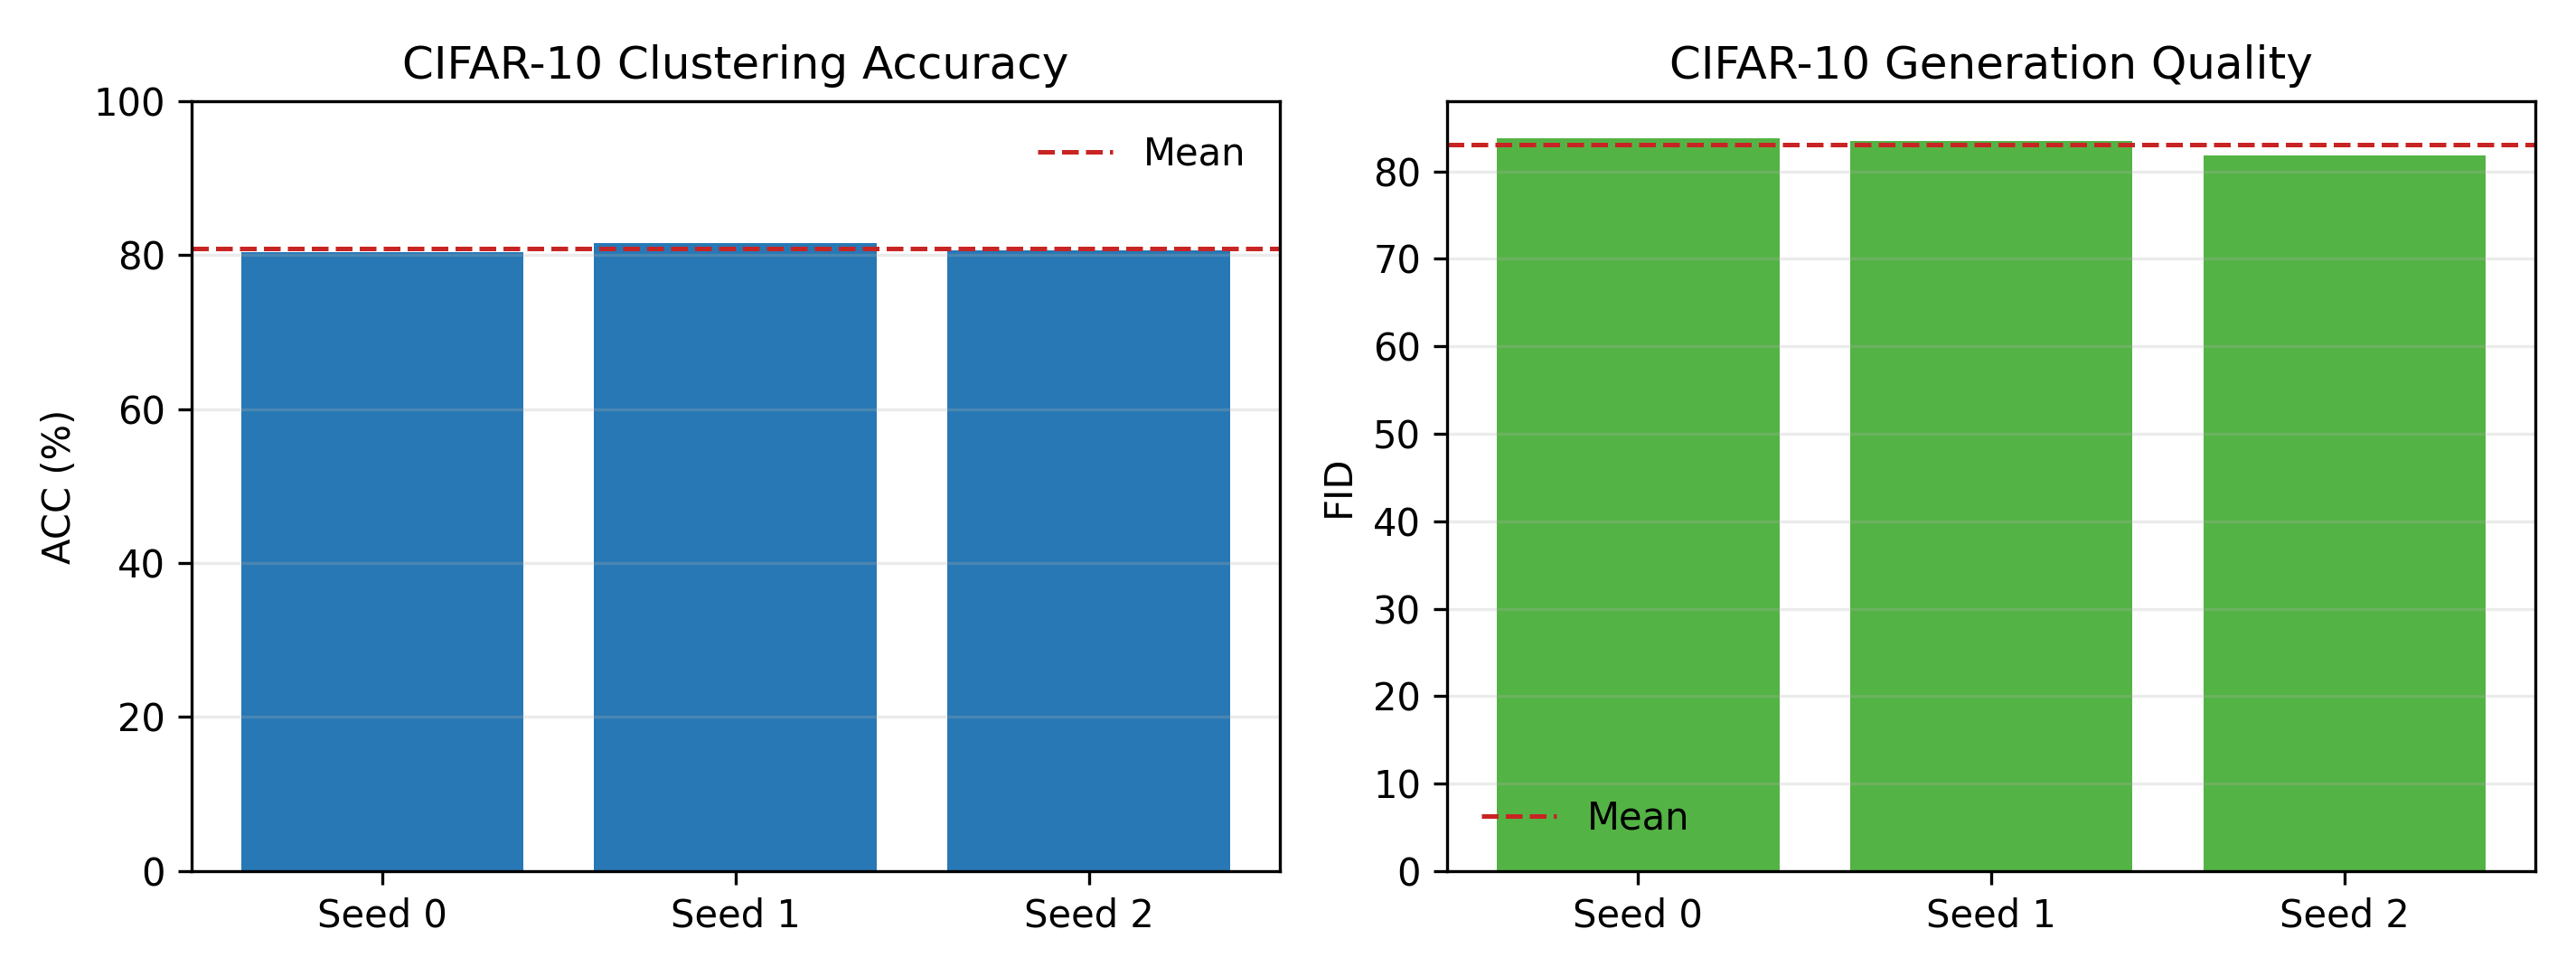
\includegraphics[width=0.92\linewidth]{cifar10_main_metrics.png}
\caption{CIFAR-10 clustering and generation metrics across the three completed \ours{} seeds.}
\label{fig:cifar-main}
\end{figure}

\subsection{CIFAR-10 Comparison to Available Baselines}

Table~\ref{tab:cifar-baselines} compares \ours{} to available local baselines. Because not all baselines have three-seed runs, the table explicitly reports the source status. The comparison should be treated as evidence for the current repository protocol rather than as a final benchmark table.

\begin{table*}[t]
\centering
\caption{Available CIFAR-10 comparison. \ours{} is a 3-seed mean; other rows are completed local seed-0 results unless marked otherwise.}
\label{tab:cifar-baselines}
\begin{tabular}{llrrrr}
\toprule
Method & Status & ACC $\uparrow$ & NMI $\uparrow$ & ARI $\uparrow$ & FID $\downarrow$ \\
\midrule
\ours{} & 3-seed mean & \textbf{0.8087} & \textbf{0.6496} & \textbf{0.6325} & \textbf{83.04} \\
\ours{} full ablation run & completed seed 0 & 0.8149 & 0.6622 & 0.6438 & 83.59 \\
ResNetAE & seed 0 & 0.2202 & 0.1017 & 0.0493 & 121.01 \\
VAE & seed 0 & 0.2220 & 0.0955 & 0.0511 & 179.98 \\
WAE-MMD & seed 0 & 0.2099 & 0.0979 & 0.0469 & 235.43 \\
VaDE & seed 0 & 0.1475 & 0.0427 & 0.0151 & 475.87 \\
\bottomrule
\end{tabular}
\end{table*}

The gap is large: \ours{} improves ACC by roughly 59 percentage points over VAE/WAE-MMD and by roughly 66 points over VaDE in this protocol. The FID gap is also favorable relative to these baselines. This is the strongest current evidence for \ours{} as a paper direction.

\begin{figure}[t]
\centering
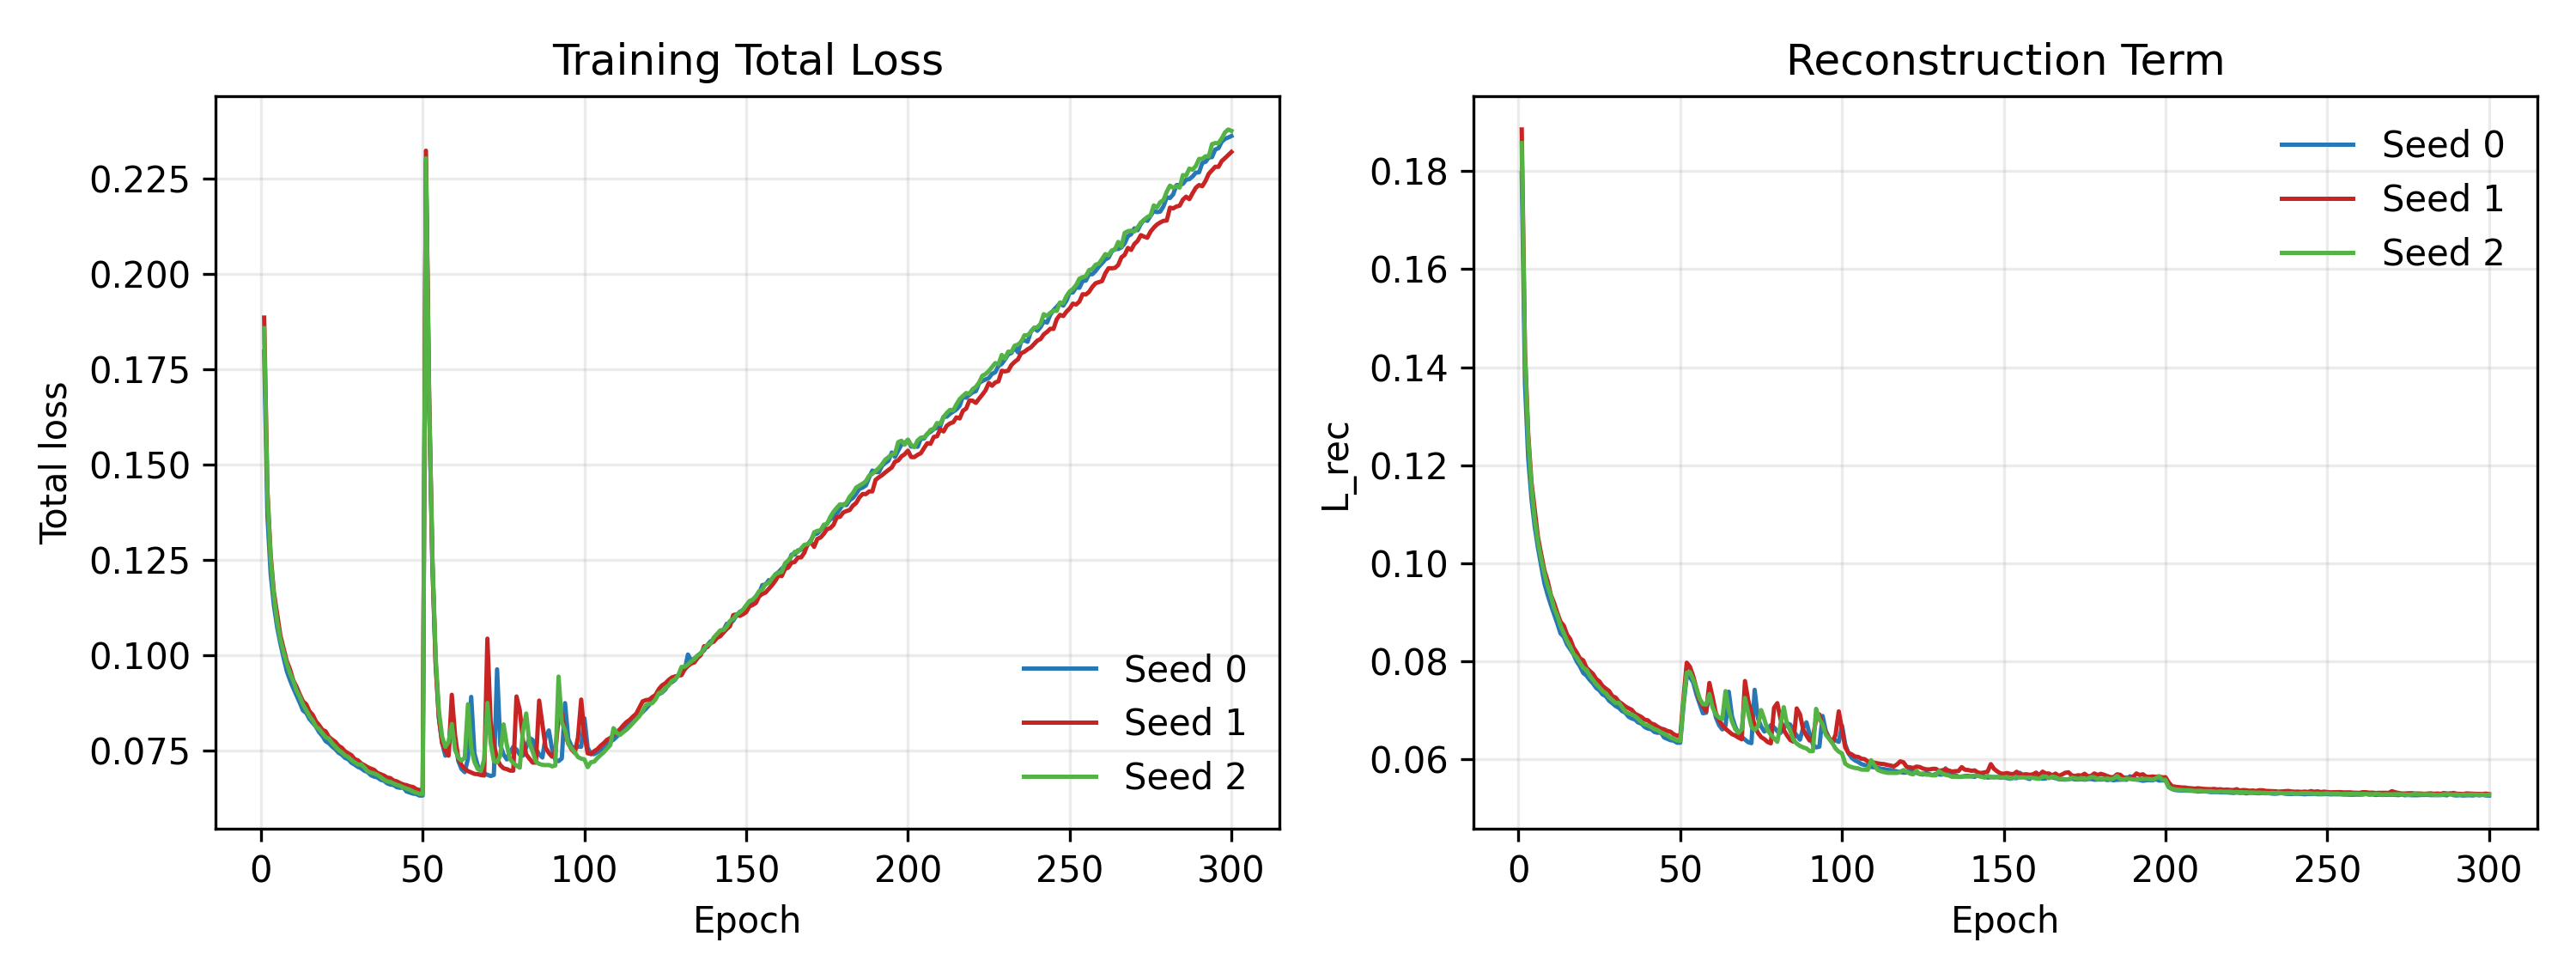
\includegraphics[width=0.95\linewidth]{cifar10_training_curves.png}
\caption{Training curves for the completed CIFAR-10 \ours{} runs. The four-phase schedule keeps training stable after style and semantic regularizers are introduced.}
\label{fig:cifar-training}
\end{figure}

\subsection{Qualitative CIFAR-10 Structure}

Figure~\ref{fig:cifar-samples} shows class-conditional prior samples from the completed CIFAR-10 checkpoint. Figure~\ref{fig:cifar-style} visualizes the intended factorization: rows with fixed semantics and varying styles, and rows with fixed style and varying semantic centers. These figures are not a substitute for quantitative ablations, but they help inspect whether the decoder uses $\zc$ and $\zs$ in a plausible way.

\begin{figure}[t]
\centering
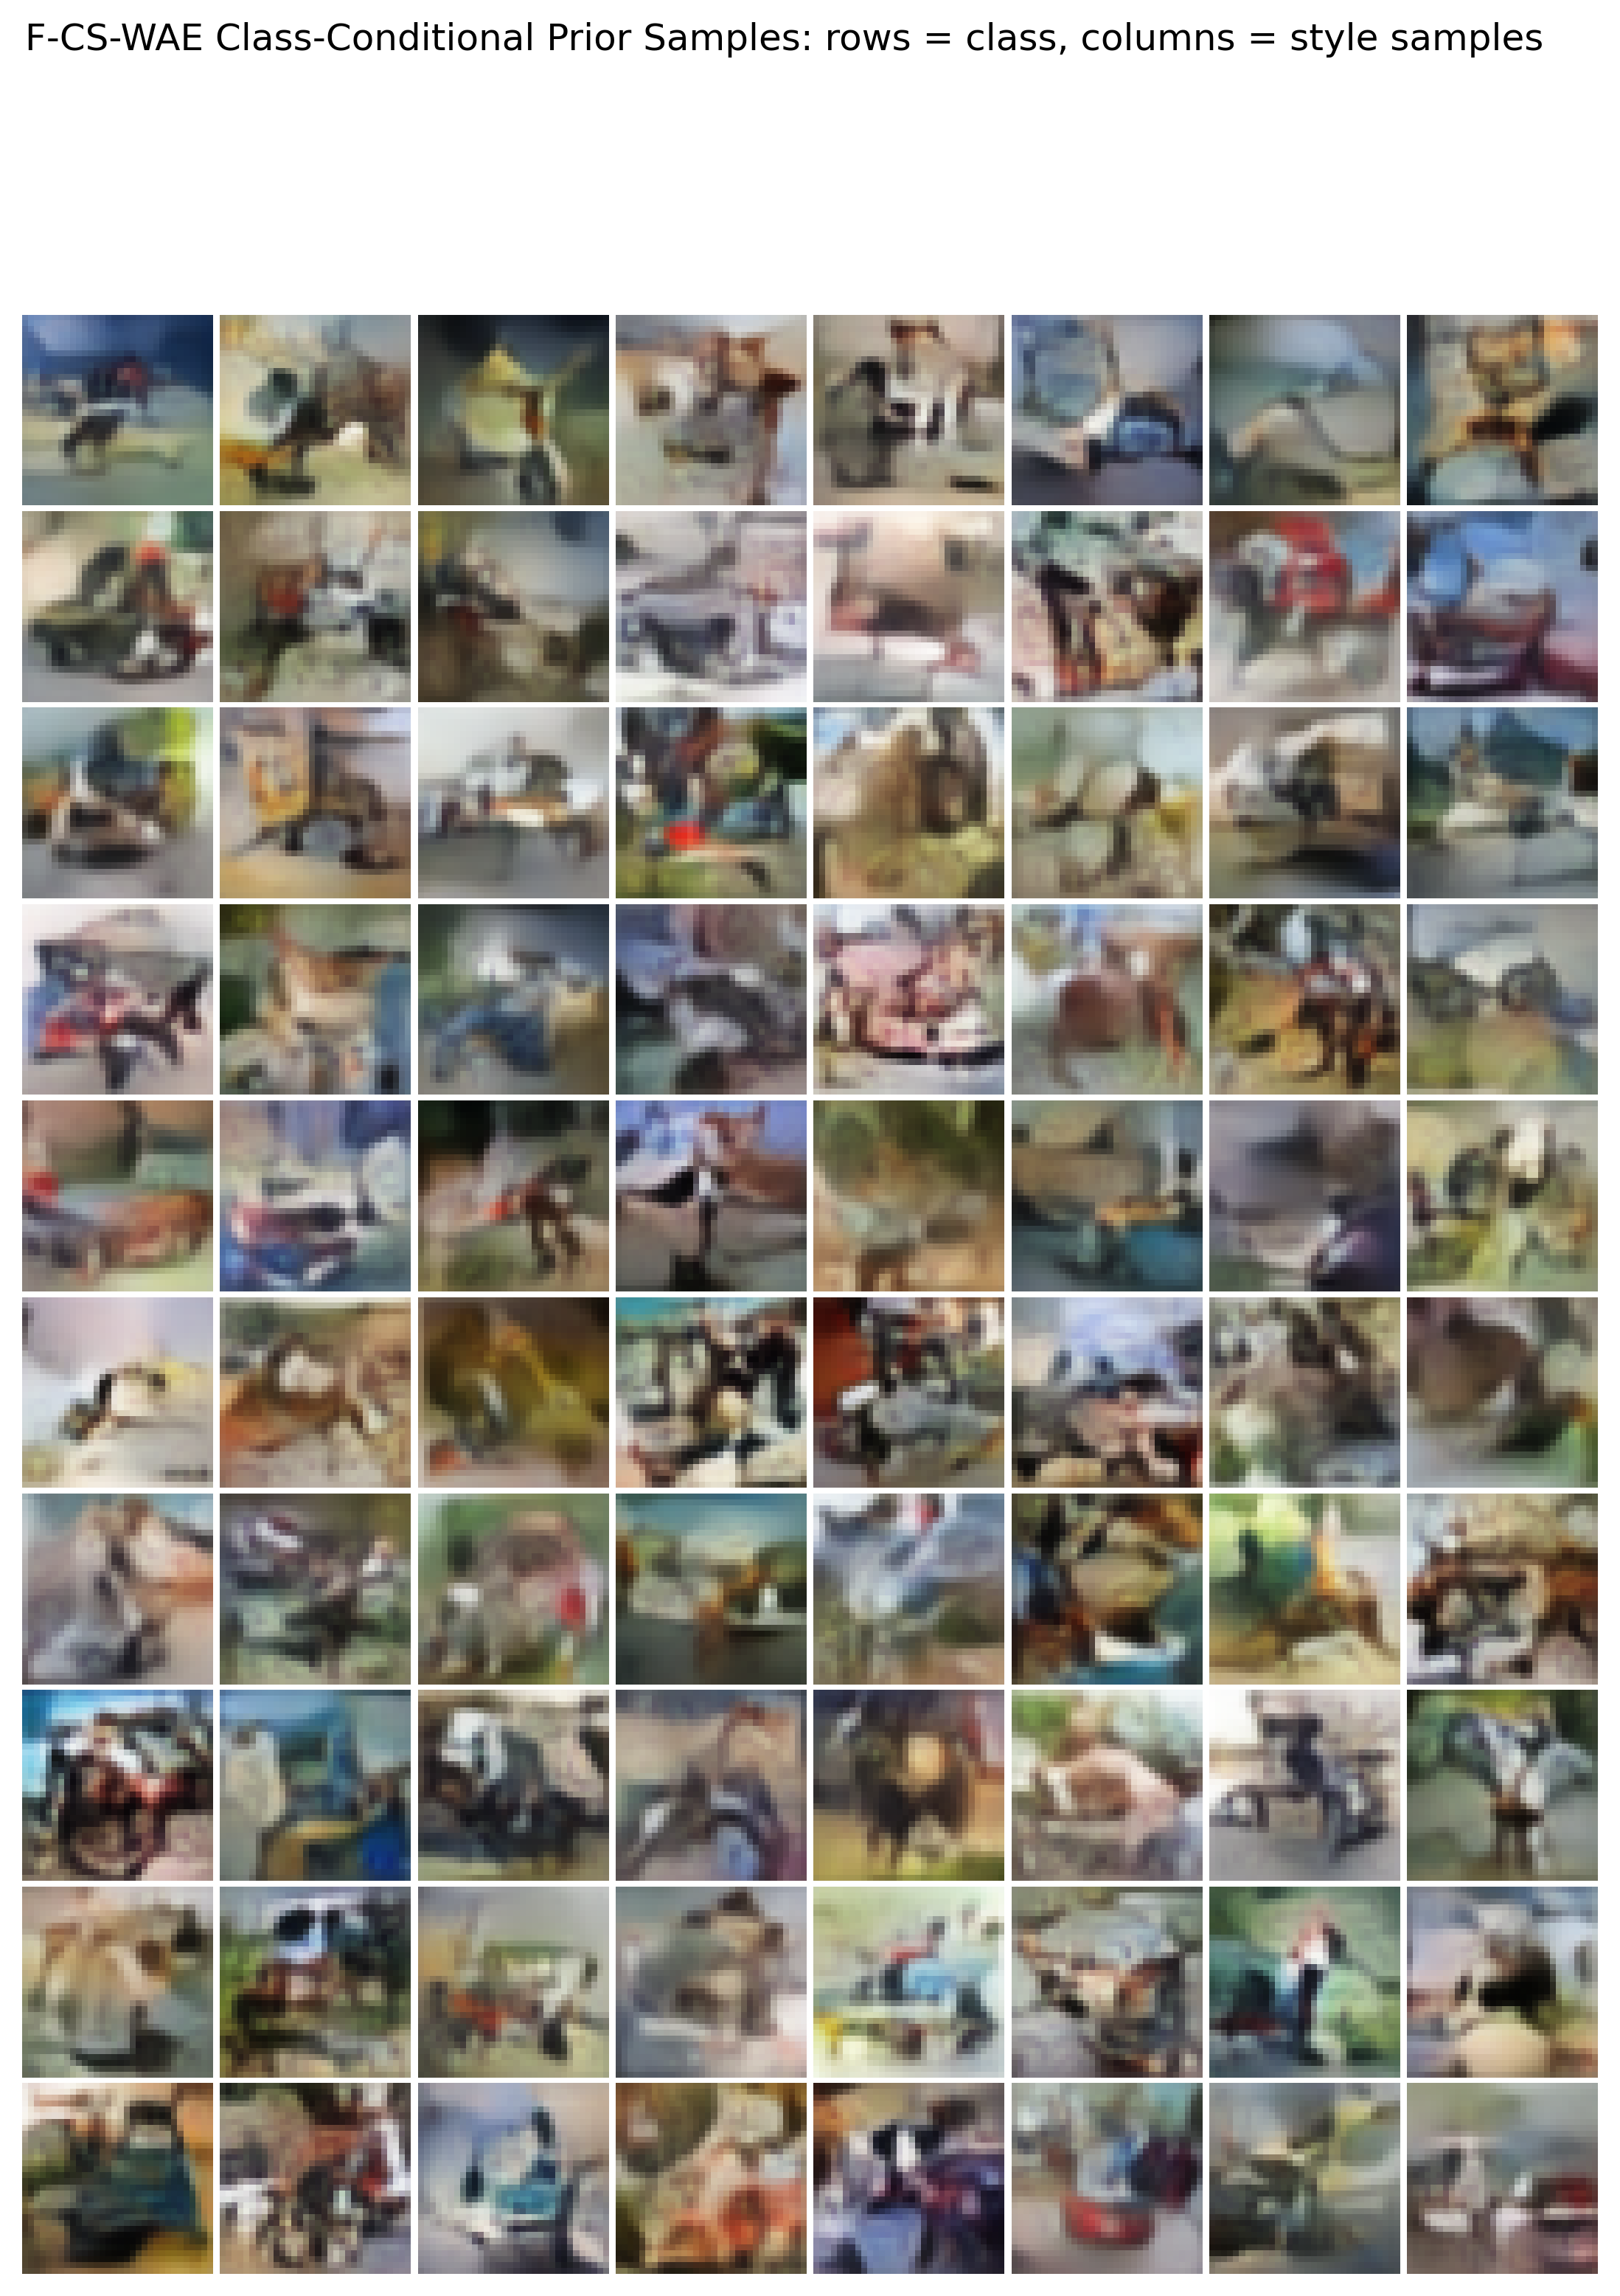
\includegraphics[width=0.95\linewidth,height=0.62\textheight,keepaspectratio]{cifar10_class_prior_grid.png}
\caption{CIFAR-10 class-conditional samples from \ours{} priors. Each row corresponds to a class prior.}
\label{fig:cifar-samples}
\end{figure}

\begin{figure}[t]
\centering
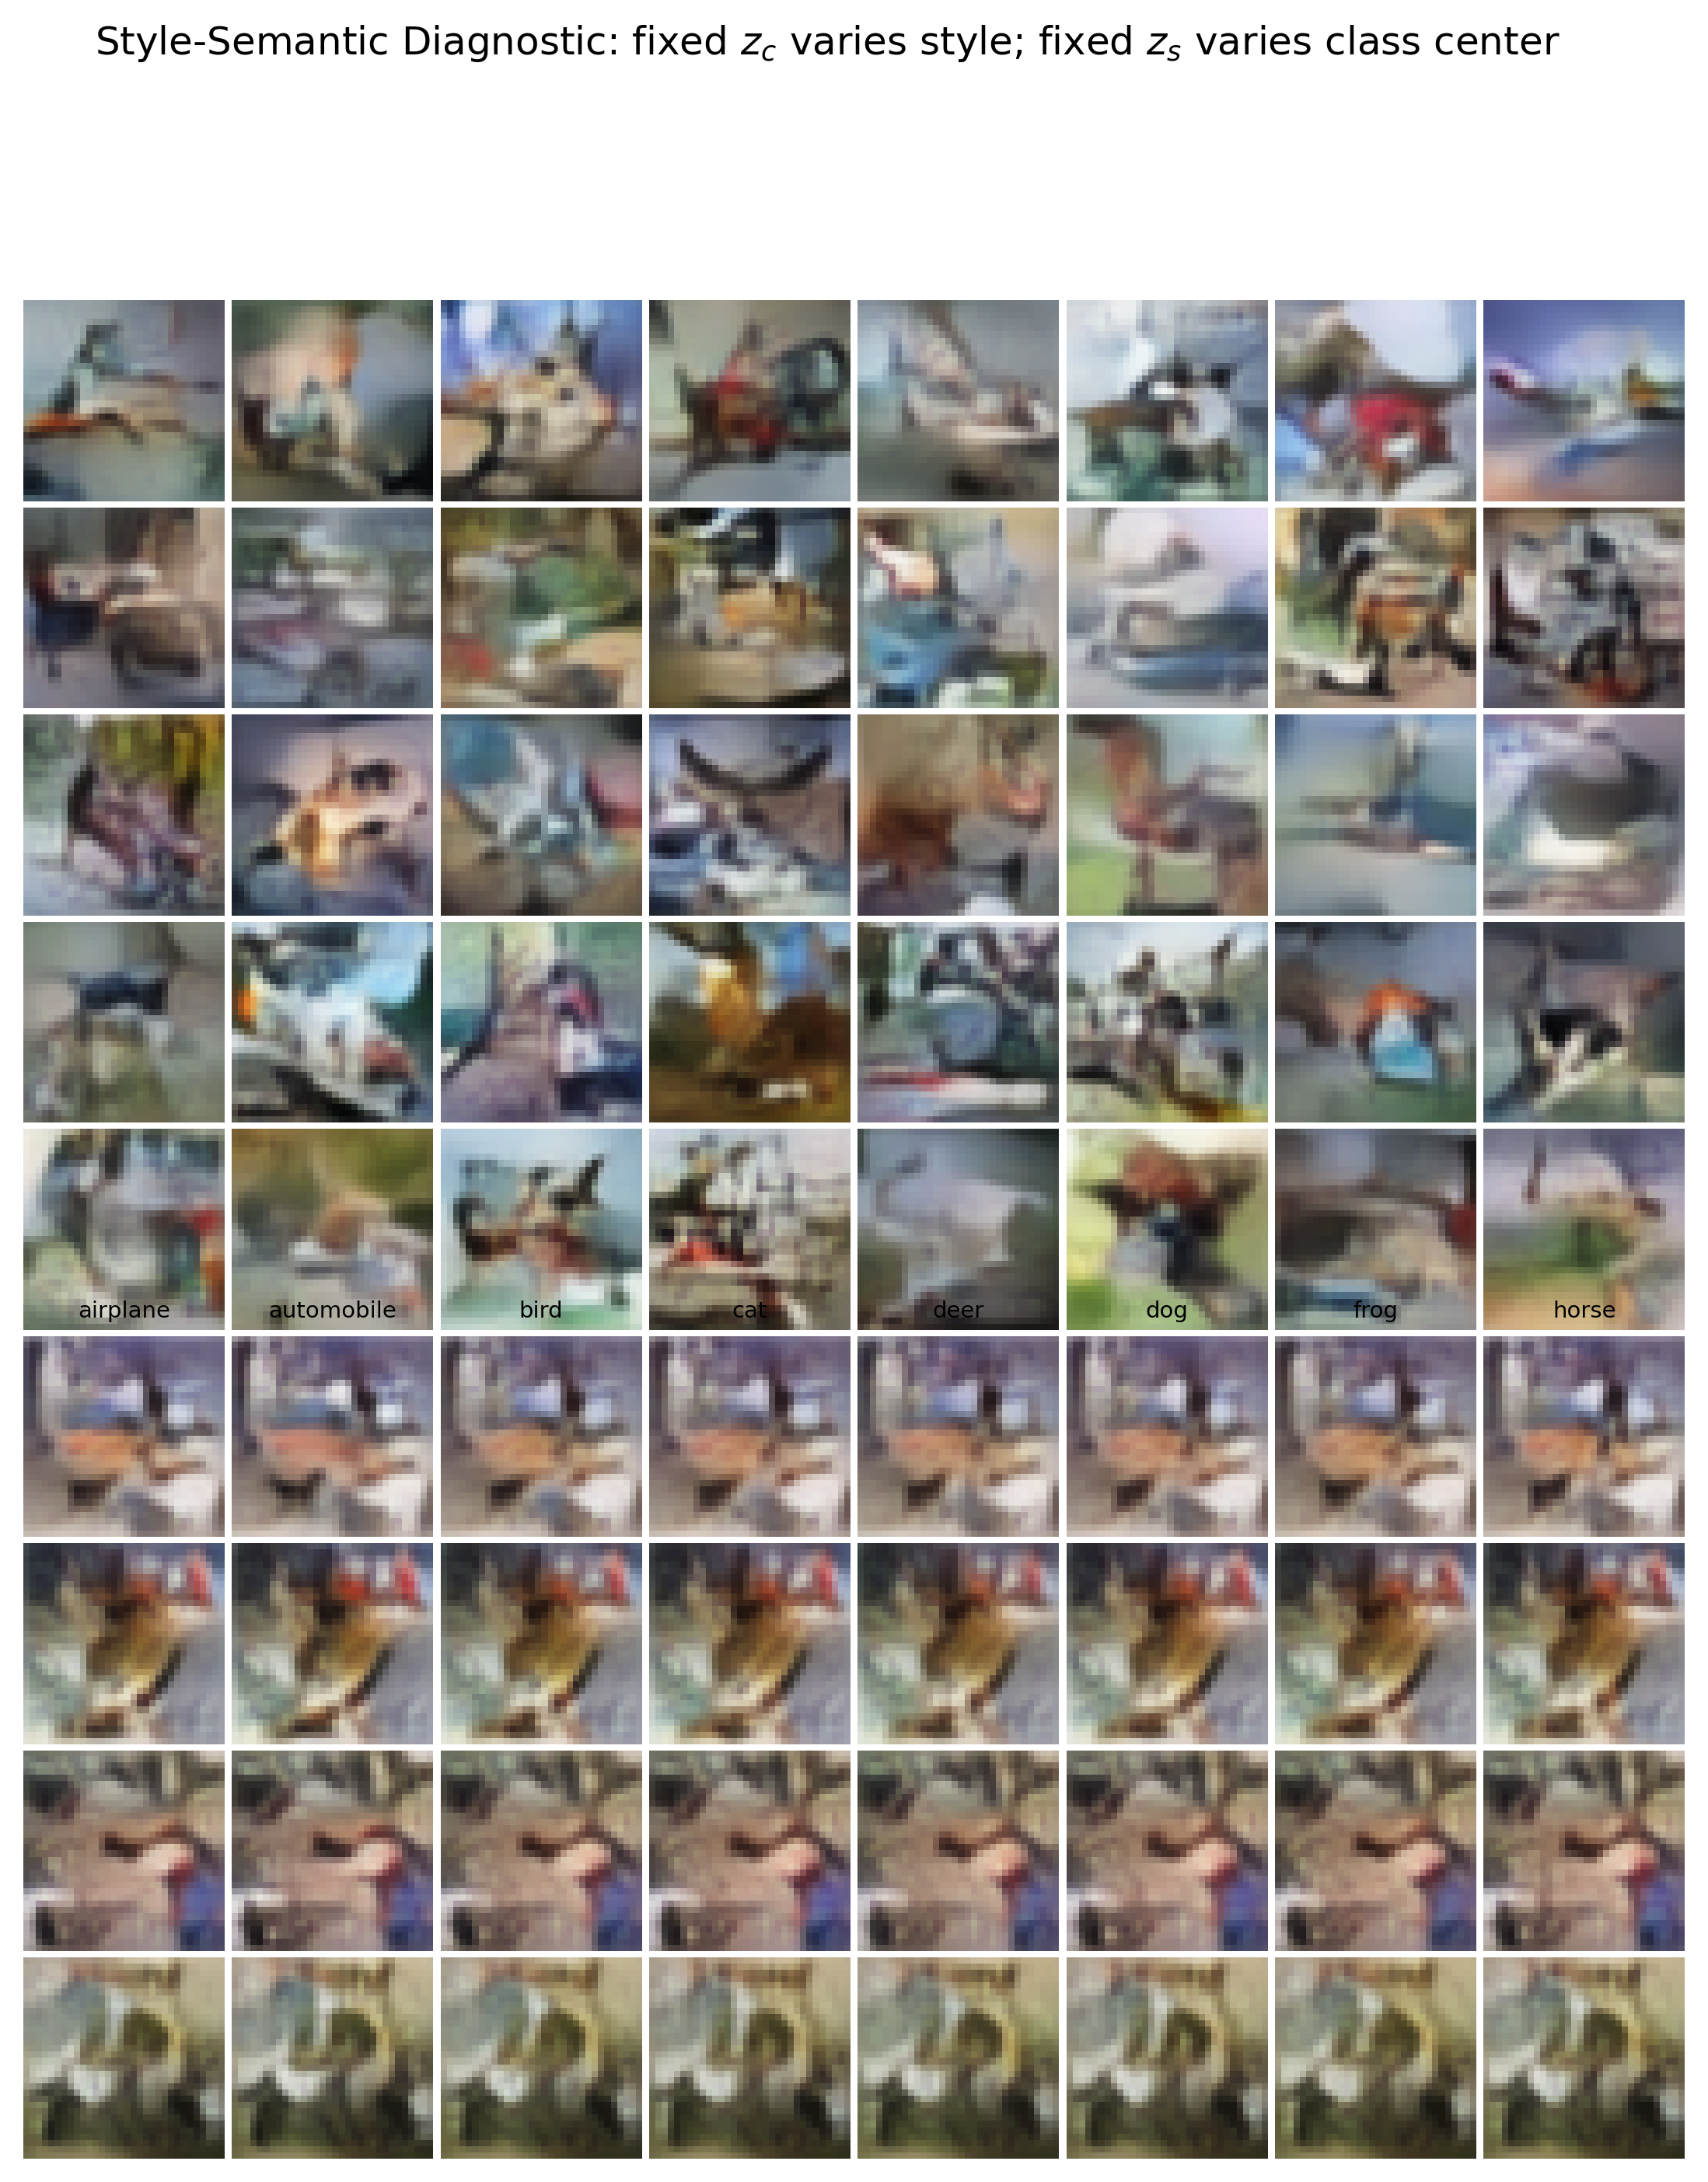
\includegraphics[width=0.95\linewidth]{cifar10_style_semantic_grid.png}
\caption{CIFAR-10 style/semantic diagnostic. The figure probes whether varying $\zs$ at fixed $\zc$, and varying $\zc$ at fixed $\zs$, produces interpretable changes.}
\label{fig:cifar-style}
\end{figure}

\subsection{MNIST: High Clustering, Poor Naive Prior Sampling}

MNIST exposes the central trade-off more sharply. Table~\ref{tab:mnist} compares \ours{} seed 0 to the single-latent \simple{} seed 0. \ours{} strongly improves clustering and reconstruction metrics, but its FID is worse. This is the key warning for an AAAI-27 submission: ACC/NMI/ARI alone would overstate the generative quality of the factorized model.

\begin{table}[t]
\centering
\caption{MNIST seed-0 comparison. \simple{} is the single-latent Spherical Cauchy WAE variant; \ours{} is the factorized model.}
\label{tab:mnist}
\begin{tabular}{lrrrrrrr}
\toprule
Method & ACC & NMI & ARI & FID & LPIPS & SSIM & PSNR \\
\midrule
\simple{} & 0.8735 & 0.8863 & 0.8411 & \textbf{26.95} & 0.0603 & 0.8127 & 16.38 \\
\ours{} & \textbf{0.9915} & \textbf{0.9758} & \textbf{0.9813} & 73.99 & \textbf{0.0120} & \textbf{0.9833} & \textbf{26.88} \\
\bottomrule
\end{tabular}
\end{table}

\begin{figure*}[t]
\centering
\begin{subfigure}[t]{0.48\linewidth}
\centering
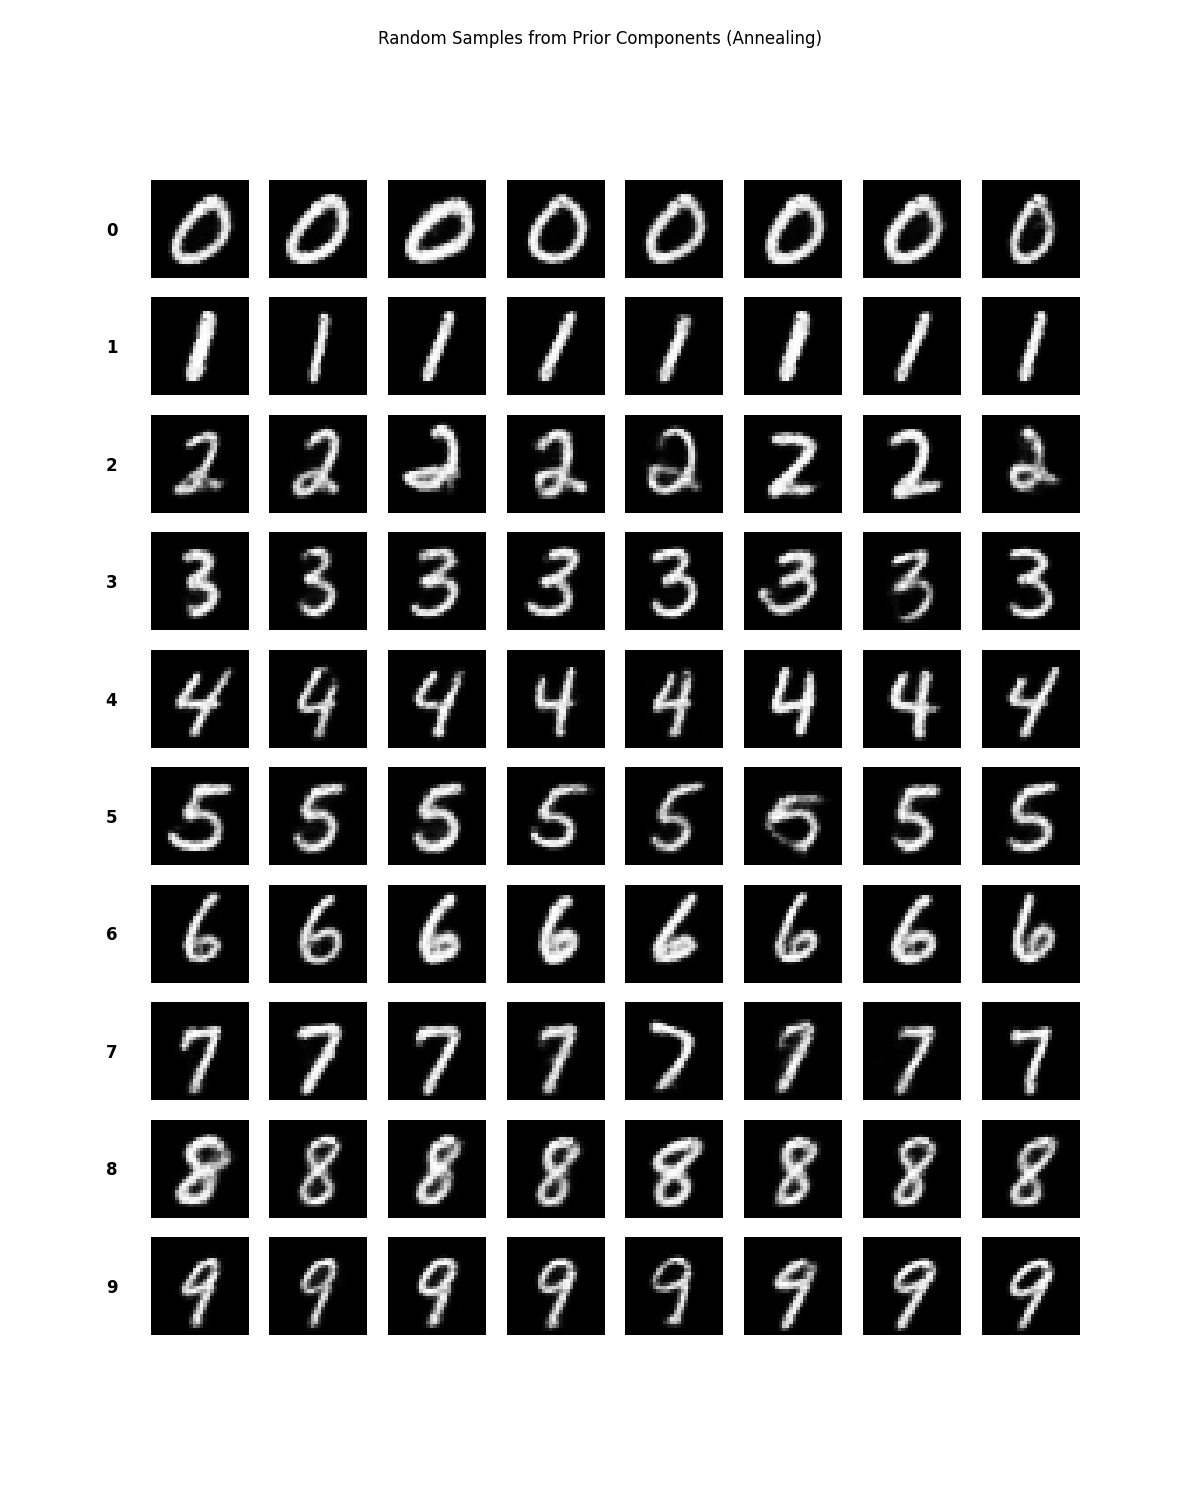
\includegraphics[width=\linewidth]{mnist_cs_prior_samples.png}
\caption{\simple{} prior samples.}
\end{subfigure}
\hfill
\begin{subfigure}[t]{0.48\linewidth}
\centering
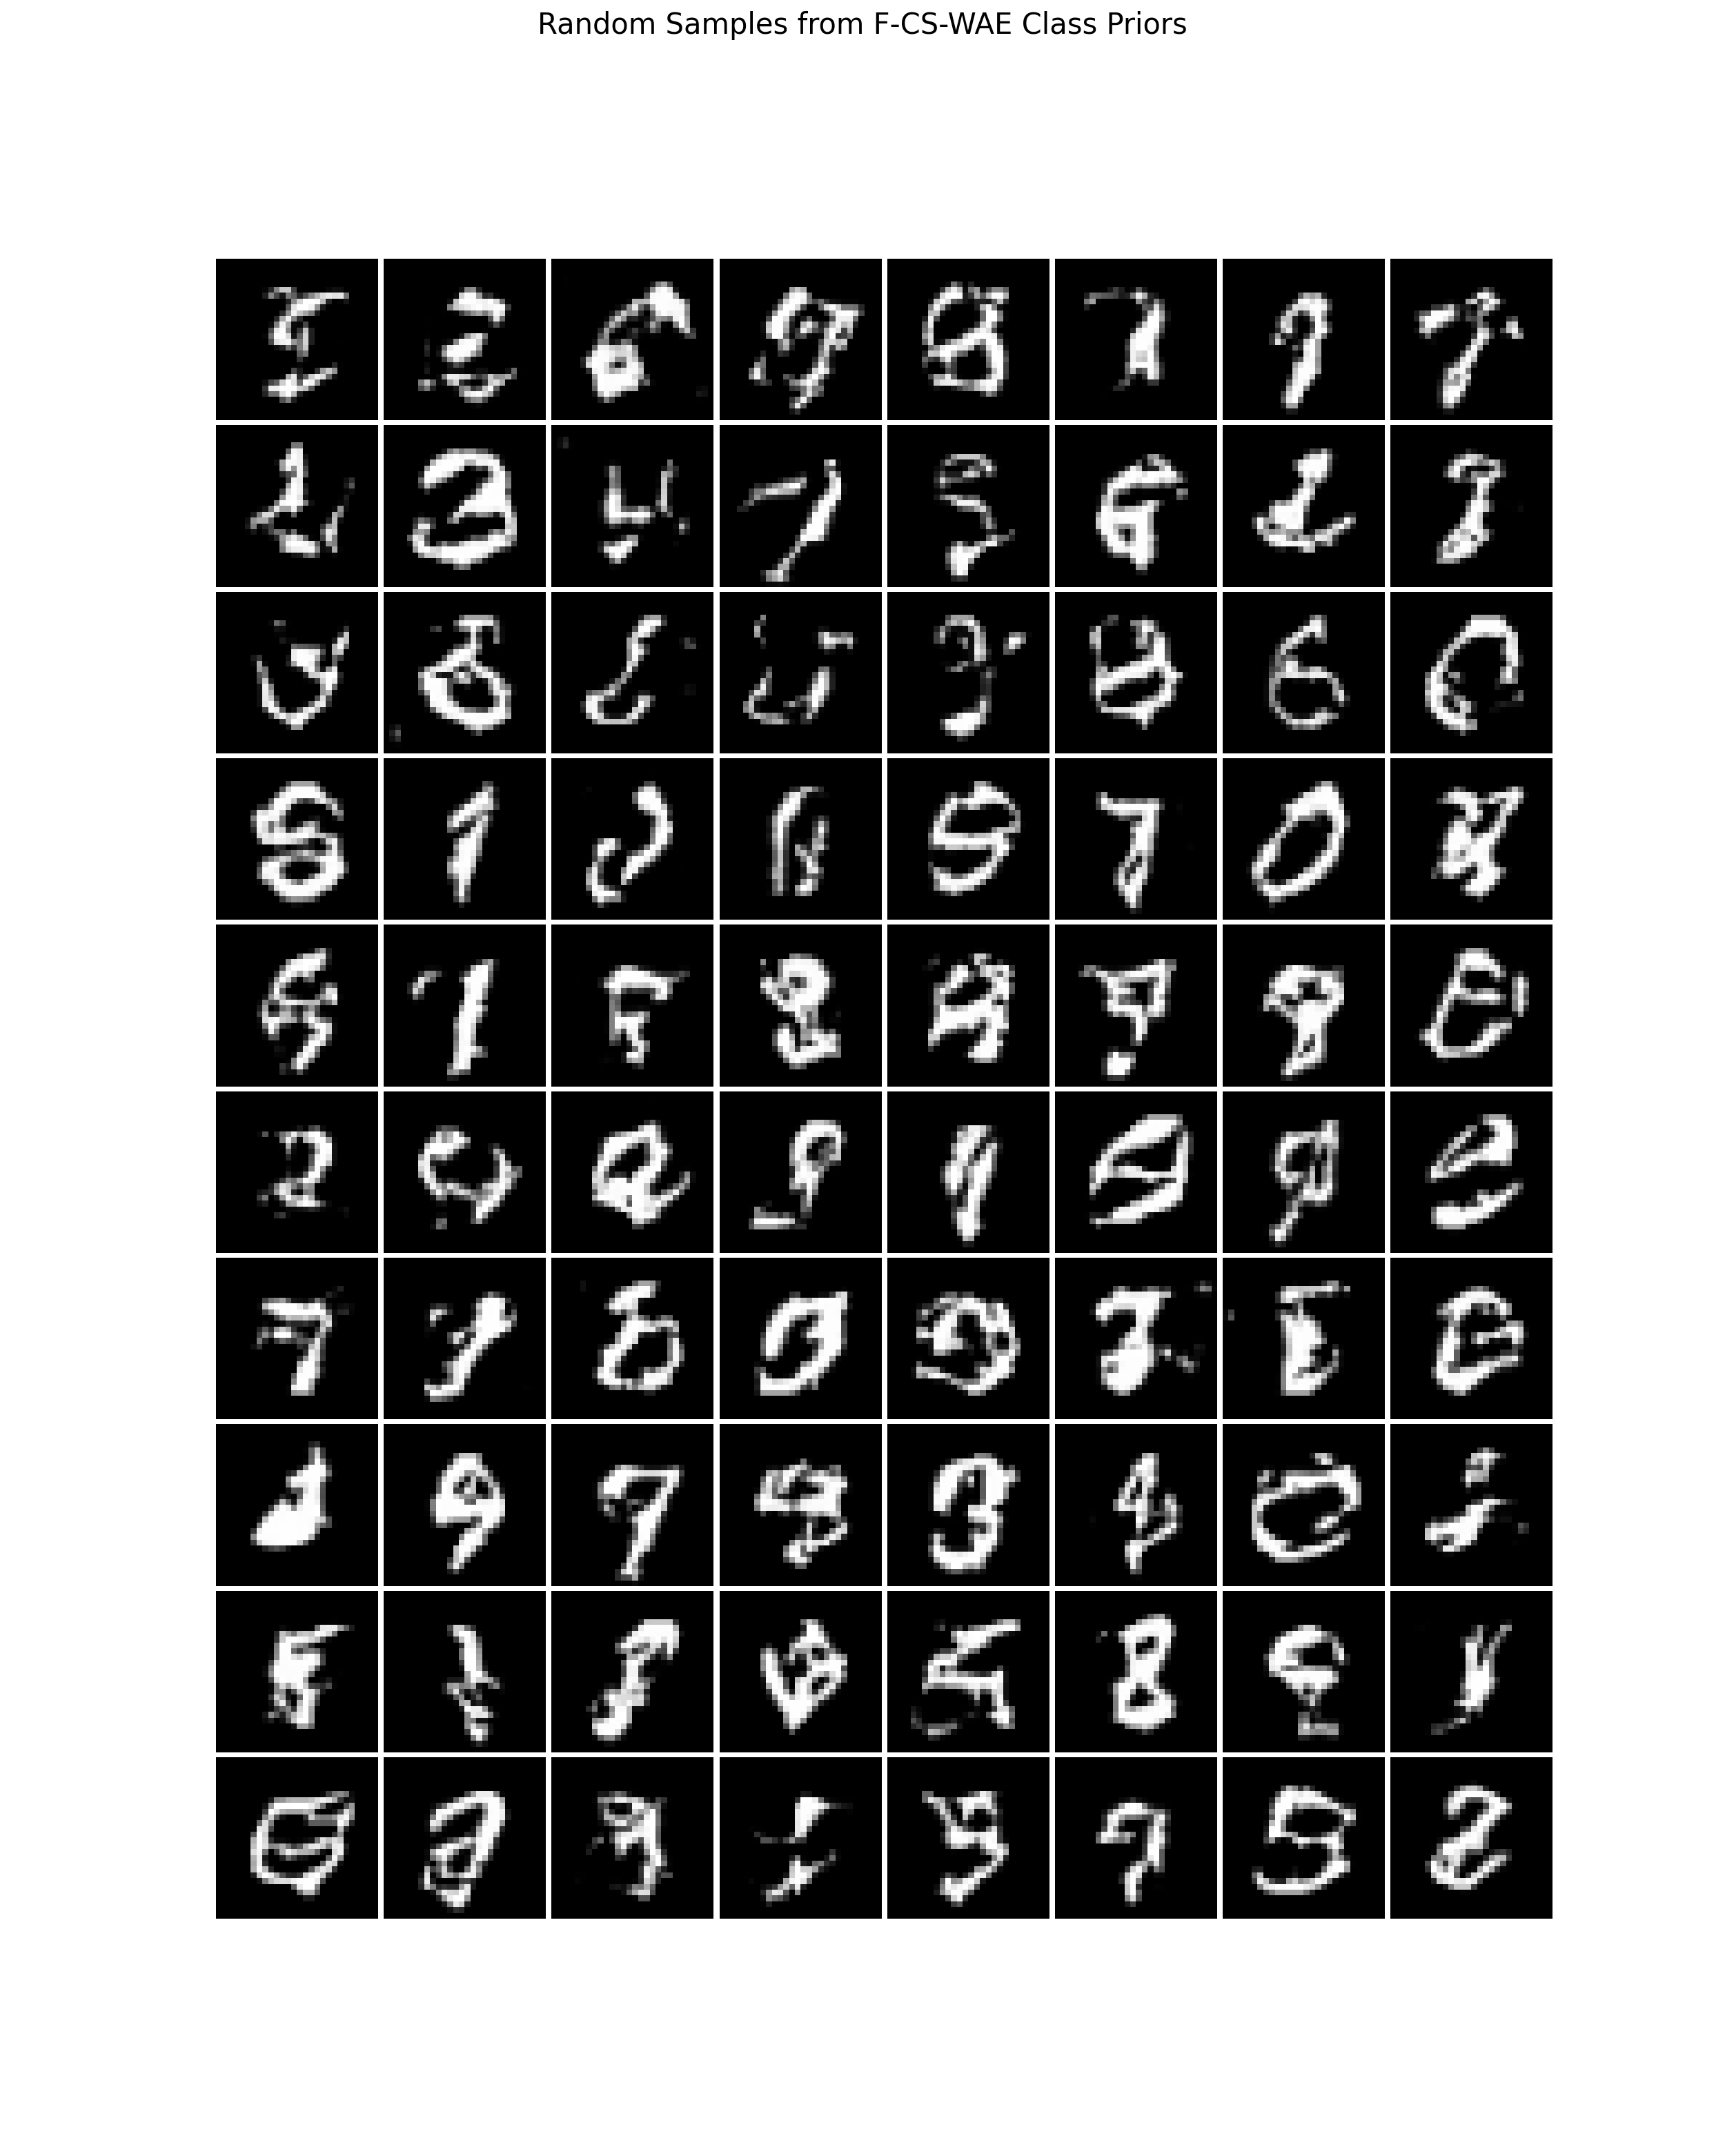
\includegraphics[width=\linewidth]{mnist_fcs_prior_samples.png}
\caption{\ours{} naive independent prior samples.}
\end{subfigure}
\caption{MNIST generation comparison. The factorized model clusters and reconstructs better, but independent sampling of $\zs\sim N(0,I)$ creates unrealistic or class-mismatched samples.}
\label{fig:mnist-prior-comparison}
\end{figure*}

\section{Failure Analysis: Conditional Style Mismatch}
\label{sec:failure}

The MNIST result raises a question: why does a model with excellent reconstruction and clustering produce poor prior samples? We tested whether the style latent is globally matched to $N(0,I)$ and whether it is independent of class. The answer is mixed.

On 2,048 MNIST test samples encoded by the \ours{} seed-0 checkpoint, the posterior style samples have global standard deviation approximately $0.989$, per-dimension variance approximately $0.973$, and multi-scale MMD to $N(0,I)$ approximately $0.0017$. By a marginal aggregate test, style matching appears successful. However, class-conditional style means remain far apart: the average pairwise distance between class style means is approximately $6.25$, while within-class style norm is approximately $10.25$. In other words, $\zs$ still carries class information.

This explains the generation failure. During training, the decoder sees pairs $(\zc,\zs)$ from the same image. If $\zs$ contains class information, then the decoder learns class-specific interactions between $\zc$ and $\zs$. During generation, the current prior samples $\zc$ from class $k$ but samples $\zs$ independently from the global Gaussian. This creates combinations that may never occur under the encoded posterior.

\begin{figure}[t]
\centering
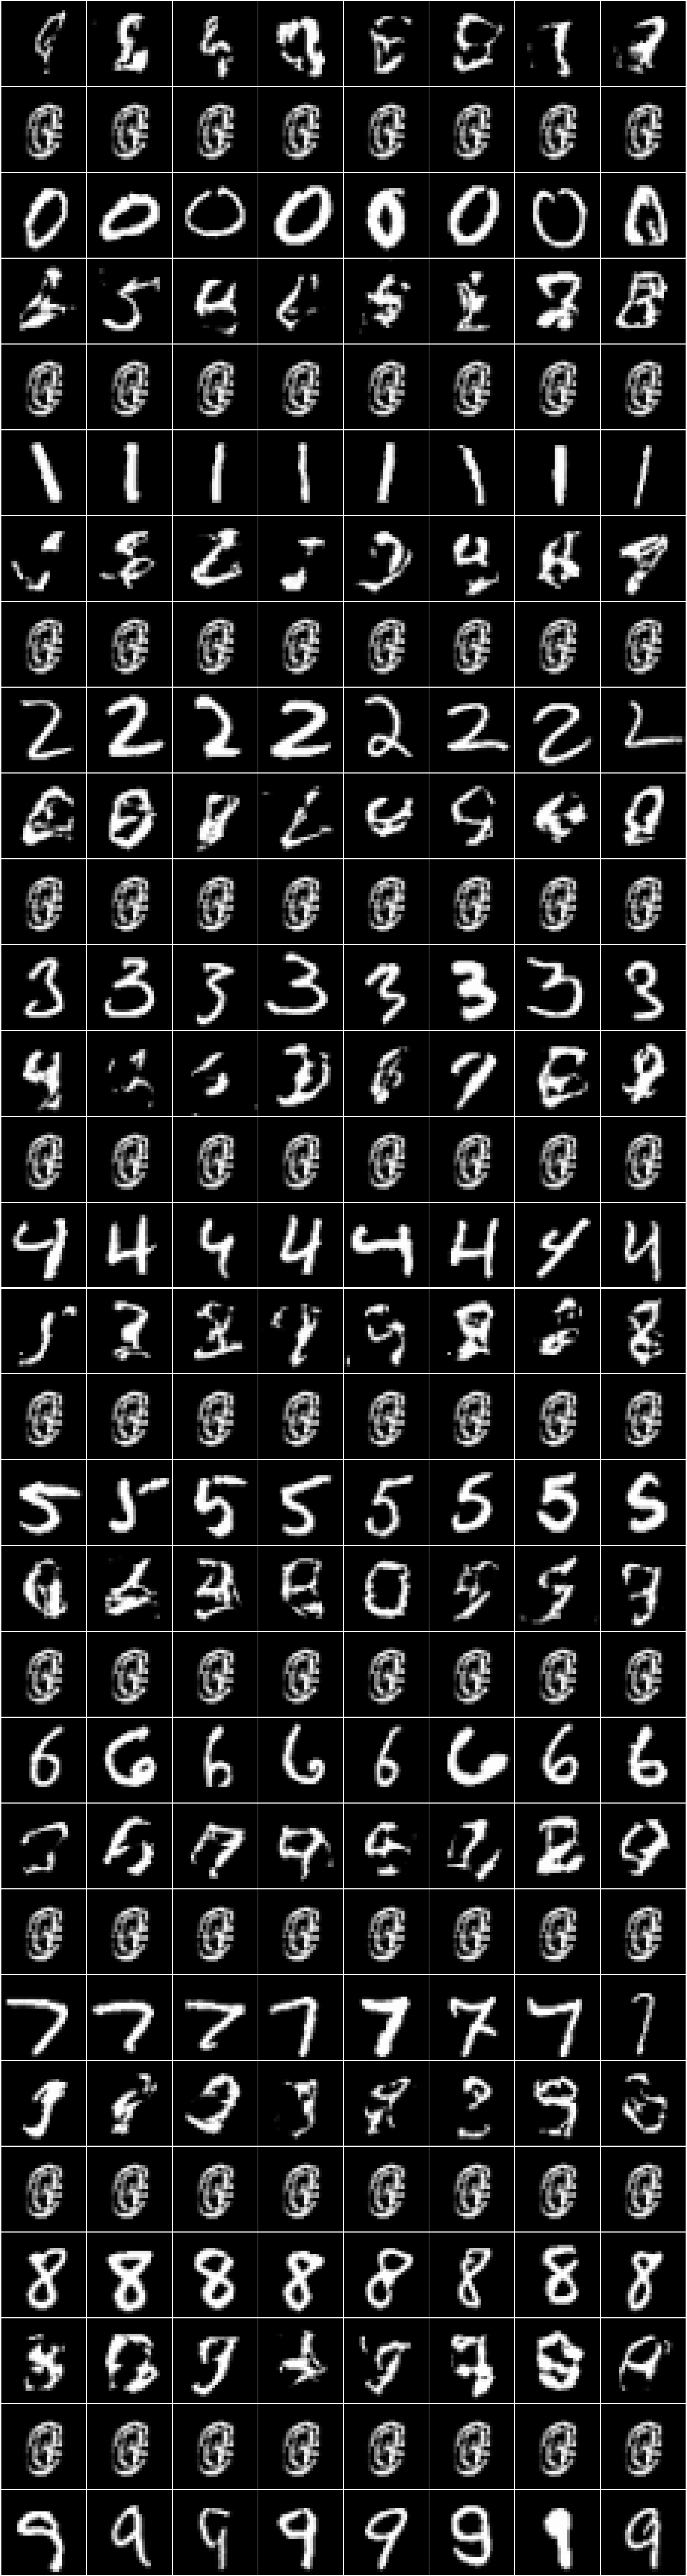
\includegraphics[width=0.68\linewidth,height=0.62\textheight,keepaspectratio]{mnist_style_prior_diagnostic.png}
\caption{MNIST style-prior diagnostic. For each digit, three rows compare $\zs\sim N(0,I)$, $\zs=0$, and empirical posterior $\zs$ sampled from the same class. Empirical same-class style codes recover clean digits; independent Gaussian style codes often decode as broken or wrong-class samples.}
\label{fig:style-diagnostic}
\end{figure}

Figure~\ref{fig:style-diagnostic} visualizes the issue. Empirical same-class style codes decode cleanly, while independent Gaussian styles often create broken samples. Setting $\zs=0$ also fails to preserve class semantics. The conclusion is direct: current \ours{} improves semantic clustering, but its intended factorization is incomplete because the style latent is not class-invariant.

\section{Toward an AAAI-27-Strength Method}
\label{sec:future}

The current draft supports the following claim: factorized semantic/style modeling can greatly improve clustering, but naive marginal style matching is insufficient for reliable class-conditional generation. For an AAAI-27 submission, the method should close this gap. We propose three concrete extensions.

\subsection{Conditional Style Prior}

Replace the independent prior $\zs\sim N(0,I)$ with a class-conditional style prior:
\begin{equation}
    \zs \sim p(\zs\mid y=k).
\end{equation}
The simplest version uses an EMA Gaussian per class:
\begin{equation}
    p(\zs\mid y=k)=N(\bar{\mu}_{s,k},\mathrm{diag}(\bar{\sigma}_{s,k}^2)).
\end{equation}
This extension matches the empirical finding that style is currently class-dependent. It is likely to improve samples quickly, but it changes the interpretation: style is no longer strictly class-independent. The paper can still make a strong claim if it frames the model as a \emph{conditional factorized prior} rather than a fully disentangled semantic/style model.

\subsection{Per-Class Style MMD}

If the goal is class-invariant style, then the loss should align each conditional style aggregate to the same Gaussian:
\begin{equation}
    \mathcal{L}_{\mathrm{style\text{-}class}}
    =
    \frac{1}{K}\sum_{k=1}^{K}
    \mathrm{MMD}\left(
        \{z_{\mathrm{s},i}:y_i=k\},
        \{\epsilon_j:\epsilon_j\sim N(0,I)\}
    \right).
\end{equation}
This directly targets the observed failure. It is stronger than global style MMD because it prevents class means from separating in style space while still matching the aggregate.

\subsection{Style Adversary or HSIC Penalty}

A complementary approach is to penalize dependence between $\zs$ and class labels. A gradient-reversal classifier can try to predict $y$ from $\zs$, while the encoder tries to make this prediction fail. Alternatively, an HSIC-style dependence penalty \citep{gretton2005measuring} can reduce dependence between $\zs$ and labels or between $\zs$ and $\zc$.

\subsection{What the Final AAAI Claim Should Be}

A paper based only on ACC/NMI/ARI would be vulnerable because the model is explicitly generative. The final AAAI-level claim should be:
\begin{quote}
    Factorized Spherical Cauchy WAE models improve label-guided clustering, but require conditional style alignment to preserve prior sample quality; with this alignment, the model achieves strong clustering and competitive generation under a unified class-conditional generative objective.
\end{quote}
This claim is stronger than a pure clustering result because it contributes both a model and a diagnosis of why factorization can fail.

\section{Discussion}

\paragraph{Why CIFAR-10 looks stronger than MNIST.}
On CIFAR-10, \ours{} improves both clustering and FID relative to the available local baselines. This likely reflects the weakness of the baselines under the same ResNet/protocol and the benefit of having a high-capacity factorized representation. On MNIST, the single-latent \simple{} prior is already well matched to the simple digit manifold, so the factorized model must justify its extra degrees of freedom. It improves clustering, but the style latent becomes an unregulated route for class information.

\paragraph{Why reconstruction is misleading.}
The MNIST \ours{} checkpoint has excellent SSIM, PSNR, and LPIPS, yet poor prior samples. This confirms a standard lesson in generative modeling: reconstruction quality is not equivalent to sample quality. A decoder can reconstruct encoded latents that lie on the posterior manifold while failing on samples from the intended prior.

\paragraph{Why the failure is useful.}
The failure is not merely a bad hyperparameter setting. It identifies a missing conditional constraint in the factorized objective. Global matching $q(\zs)\approx N(0,I)$ does not imply $q(\zs\mid y=k)\approx N(0,I)$ for all $k$, nor does it imply $\zs\perp y$. This is precisely the gap that conditional style priors or per-class style MMD should close.

\paragraph{Limitations of the current draft.}
The completed evidence is not yet sufficient for a final AAAI-27 submission. CIFAR-10 has strong three-seed results, but MNIST and Fashion-MNIST need full multi-seed factorized runs. Ablations are incomplete. The conditional style fix proposed in Section~\ref{sec:future} must be implemented and evaluated. The current paper draft is therefore a detailed research manuscript and submission plan, not a finished empirical package.

\section{Conclusion}

We presented \ours, a factorized class-structured Spherical Cauchy WAE for label-guided generative clustering. The model separates semantic and style latents, aligns semantics with hyperspherical class priors, and regularizes style toward a Gaussian prior through MMD. Completed CIFAR-10 experiments show strong and stable clustering performance with favorable generation metrics relative to available baselines. MNIST diagnostics reveal a deeper issue: marginal style matching can hide class dependence in the style latent, causing naive independent prior samples to decode poorly.

The main lesson is that factorization is not obtained by architectural separation alone. A factorized generative model needs conditional distributional constraints that match how sampling will be performed. For an AAAI-27-strength submission, the next step is therefore clear: preserve the clustering gains of \ours{} while adding conditional style alignment to make class-conditional generation reliable.

\bibliographystyle{plainnat}
\bibliography{references}

\appendix

\section{Repository Artifacts Used}

All quantitative claims in this draft are taken from local repository artifacts:
\begin{itemize}
    \item CIFAR-10 \ours{} metrics: \texttt{runs\_f/cifar10/seed\_\{0,1,2\}/metrics.json}.
    \item CIFAR-10 summary tables and figures: \texttt{paper\_outputs/f\_cs\_wae\_cifar10/}.
    \item MNIST \ours{} metrics and images: \texttt{runs\_f/mnist/seed\_0/}.
    \item MNIST \simple{} metrics and images: \texttt{runs/mnist/seed\_0/}.
\end{itemize}

\section{AAAI-27 Submission Checklist}

Before submission, the following experiments should be completed:
\begin{itemize}
    \item Run \ours{} on MNIST and Fashion-MNIST for seeds 0, 1, 2.
    \item Implement conditional style prior and per-class style MMD.
    \item Run ablations: no style latent, no semantic MMD, no style MMD, no auxiliary classifier, conditional style prior, per-class style MMD, style adversary, style dimension sweep.
    \item Recompute all FID directories after changing sampling.
    \item Add a final benchmark table with matched seeds for all baselines.
    \item Replace this preamble with the official AAAI-27 author kit.
\end{itemize}

\end{document}
